\chapter{Análisis}

\section{Introducción}


\section{Diagrama de Casos de Uso}
El diagrama de casos de uso es una forma de representar los requerimientos de un sistema, cada caso de uso reune una serie de requisitos basandose en diferemtes funciones o tareas.
\\
\\
Actor: Es una agrupacion uniforme de personas, sistemas o maquinas que interactuan con el sistema que estamos construyendo.   
Caso de Uso: Son secuencias de interacciones entre actores y un sistema que usan un servicio. 

\begin{figure}[th!]
	\centering
	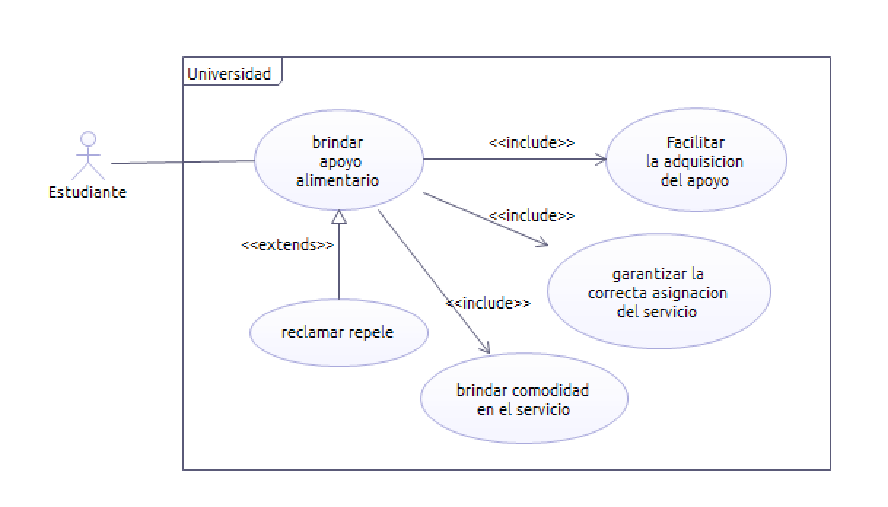
\includegraphics[width=0.8\linewidth]{uml/caso1}
	\caption{caso1}
	\label{fig:caso1}
\end{figure}

\begin{table}[]
\centering
\caption{Caso de Uso CU-1}
\label{my-label}
\begin{tabular}{|l|l|}
\hline
\textbf{Nombre}      & Brindar Apoyo Alimentario                                                                                                                                                   \\ \hline
\textbf{Actores}     & Estudiantes                                                                                                                                                                 \\ \hline
\textbf{Escenario}   &                                                                                                                                                                             \\ \hline
\textbf{Primario}    & Brindar Apoyo Alimentario                                                                                                                                                   \\ \hline
\textbf{Secundario}  & No coinciden Horarios                                                                                                                                                       \\ \hline
\textbf{Excepciones} & \begin{tabular}[c]{@{}l@{}}Solicitud de Inscripción no aceptada, Estudiante no Registrado,\\ Se acabo el alimento, Ser retirado del beneficio por alguna falla\end{tabular} \\ \hline
\end{tabular}
\end{table}

\begin{table}[]
\centering
\caption{Caso de Uso CU-2}
\label{my-label}
\begin{tabular}{|l|l|}
\hline
\textbf{Nombre}      & Reclamar Repele                                                                                                                                          \\ \hline
\textbf{Actores}     & Estudiantes                                                                                                                                              \\ \hline
\textbf{Escenario}   &                                                                                                                                                          \\ \hline
\textbf{Primario}    & Reclamar Repele                                                                                                                                          \\ \hline
\textbf{Secundario}  &                                                                                                                                                          \\ \hline
\textbf{Excepciones} & \begin{tabular}[c]{@{}l@{}}No sobro alimento, Estudiante no Registrado, Ser retirado del beneficio,\\ La hora del reclamo no es la adecuada\end{tabular} \\ \hline
\end{tabular}
\end{table}

\begin{table}[]
\centering
\caption{Caso de Uso CU-3}
\label{my-label}
\begin{tabular}{|l|l|}
\hline
\textbf{Nombre}      & Brindar Comodidad en el Servicio                                                                                                                                            \\ \hline
\textbf{Actores}     & Administrativos, Estudiantes                                                                                                                                                \\ \hline
\textbf{Escenario}   &                                                                                                                                                                             \\ \hline
\textbf{Primario}    & Brindar Comodidad en el Servicio                                                                                                                                            \\ \hline
\textbf{Secundario}  & Presentar Inscripción en la fechas no estipuladas                                                                                                                           \\ \hline
\textbf{Excepciones} & \begin{tabular}[c]{@{}l@{}}Se presenta algún error en la Infreestructura, No se abríran convocatorias\\ No se cuentan con los espacios o horarios disponibles.\end{tabular} \\ \hline
\end{tabular}
\end{table}

\begin{table}[]
\centering
\caption{Casso de Uso CU-4}
\label{my-label}
\begin{tabular}{|l|l|}
\hline
\textbf{Nombre}      & Garantizar Correcta Asignación del Servicio                                                                                                                                                                                       \\ \hline
\textbf{Actores}     & Empleados y Administrativos encargados del apoyo                                                                                                                                                                                  \\ \hline
\textbf{Escenario}   &                                                                                                                                                                                                                                   \\ \hline
\textbf{Primario}    & Garantizar Correcta Asignación del Servicio                                                                                                                                                                                       \\ \hline
\textbf{Secundario}  & \begin{tabular}[c]{@{}l@{}}Presentarse en las horas no adecuadas, Presentar alguna inconveniente\\ en un requerimiento del Apoyo\end{tabular}                                                                                     \\ \hline
\textbf{Excepciones} & \begin{tabular}[c]{@{}l@{}}Fallos en la Infreestructura, Falla del Personal encargado de brindar\\ el servicio, Inconvenientes presentados tanto en espacios como\\ horarios habilitados para la entrega del servicio\end{tabular} \\ \hline
\end{tabular}
\end{table}

\begin{table}[]
\centering
\caption{Caso de Uso CU-5}
\label{my-label}
\begin{tabular}{|l|l|}
\hline
\textbf{Nombre}      & Facilitar Adquisición del Apoyo                                                                                                                                                      \\ \hline
\textbf{Actores}     & Administrativos, Personal encargado de brindar el servicio                                                                                                                           \\ \hline
\textbf{Escenario}   &                                                                                                                                                                                      \\ \hline
\textbf{Primario}    & Facilitar Adquisión del Apoyo                                                                                                                                                        \\ \hline
\textbf{Secundario}  & Presentar alguna inconsistencia en la inscripción o documentos que soportan la misma,                                                                                                \\ \hline
\textbf{Excepciones} & \begin{tabular}[c]{@{}l@{}}Fallos en la Infreestructura, No poder optar por el beneficio por falta de cupos,\\ No tener el puntaje necesarios para recibir el beneficio\end{tabular} \\ \hline
\end{tabular}
\end{table}

\clearpage
% Please add the following required packages to your document preamble:
% \usepackage[table,xcdraw]{xcolor}
% If you use beamer only pass "xcolor=table" option, i.e. \documentclass[xcolor=table]{beamer}

\newpage

%%\section{Interacciones}

%%\newpage

\subsection{Diagrama de Secuencia}
	\begin{figure}[th!]
		\centering
		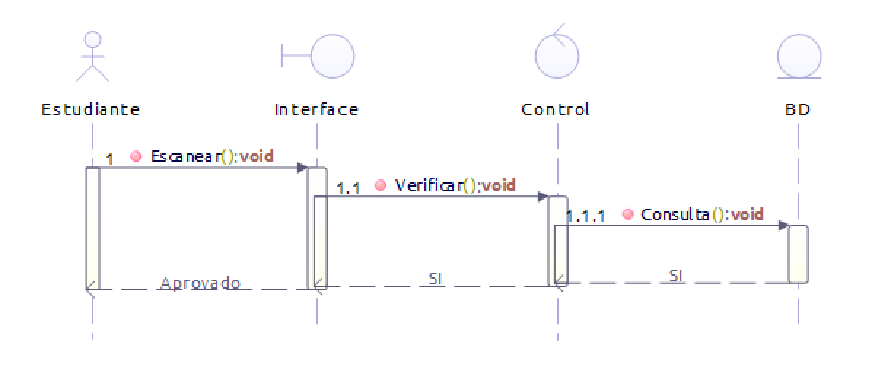
\includegraphics[width=0.9\linewidth]{uml/Asistencia}
		\caption{Diagrama de Asistencia}
		\label{fig:Diagrama de Asistencia}
	\end{figure}

	\begin{figure}[th!]
	\centering
	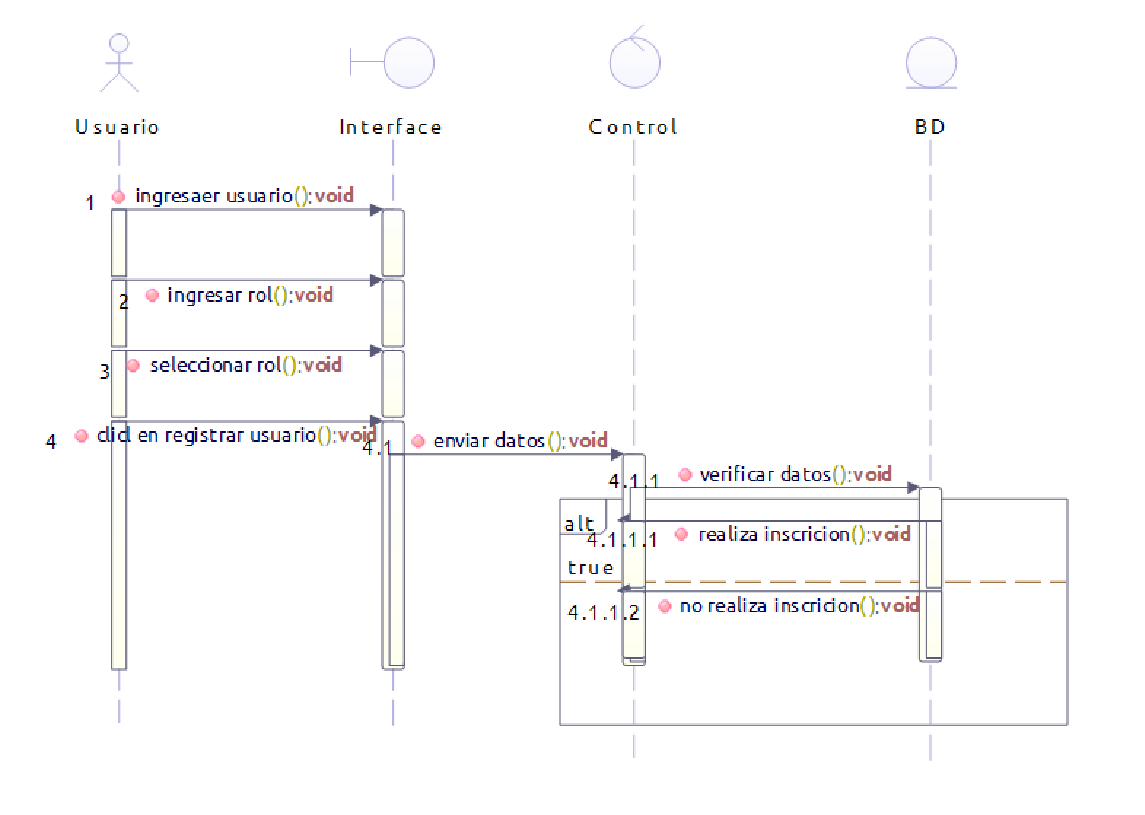
\includegraphics[width=1.1\linewidth]{uml/RegUsu}
	\caption{Registro del Usuario}
	\label{fig:Registro del Usuario}
	\end{figure}

	\begin{figure}[th!]
	\centering
	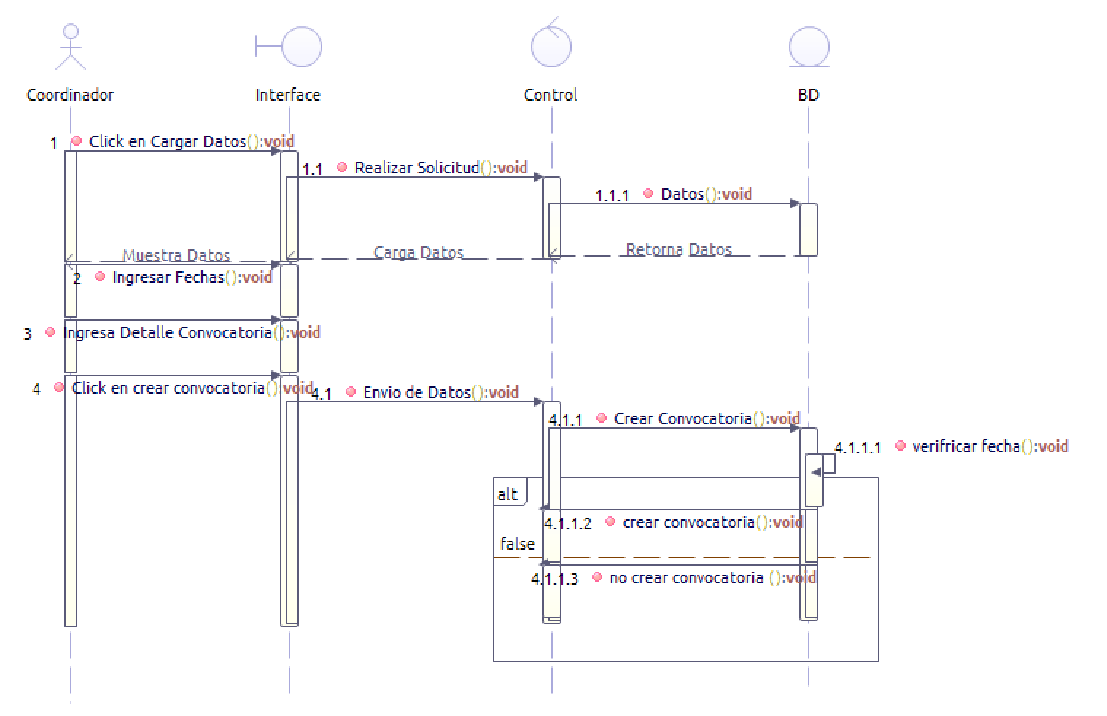
\includegraphics[width=1.4\linewidth]{uml/SecCrearConv}
	\caption{Crear convocatio del apoyo}
	\label{fig:Crear convocatio del apoyo}
	\end{figure}
\clearpage
	\begin{figure}[th!]
	\centering
	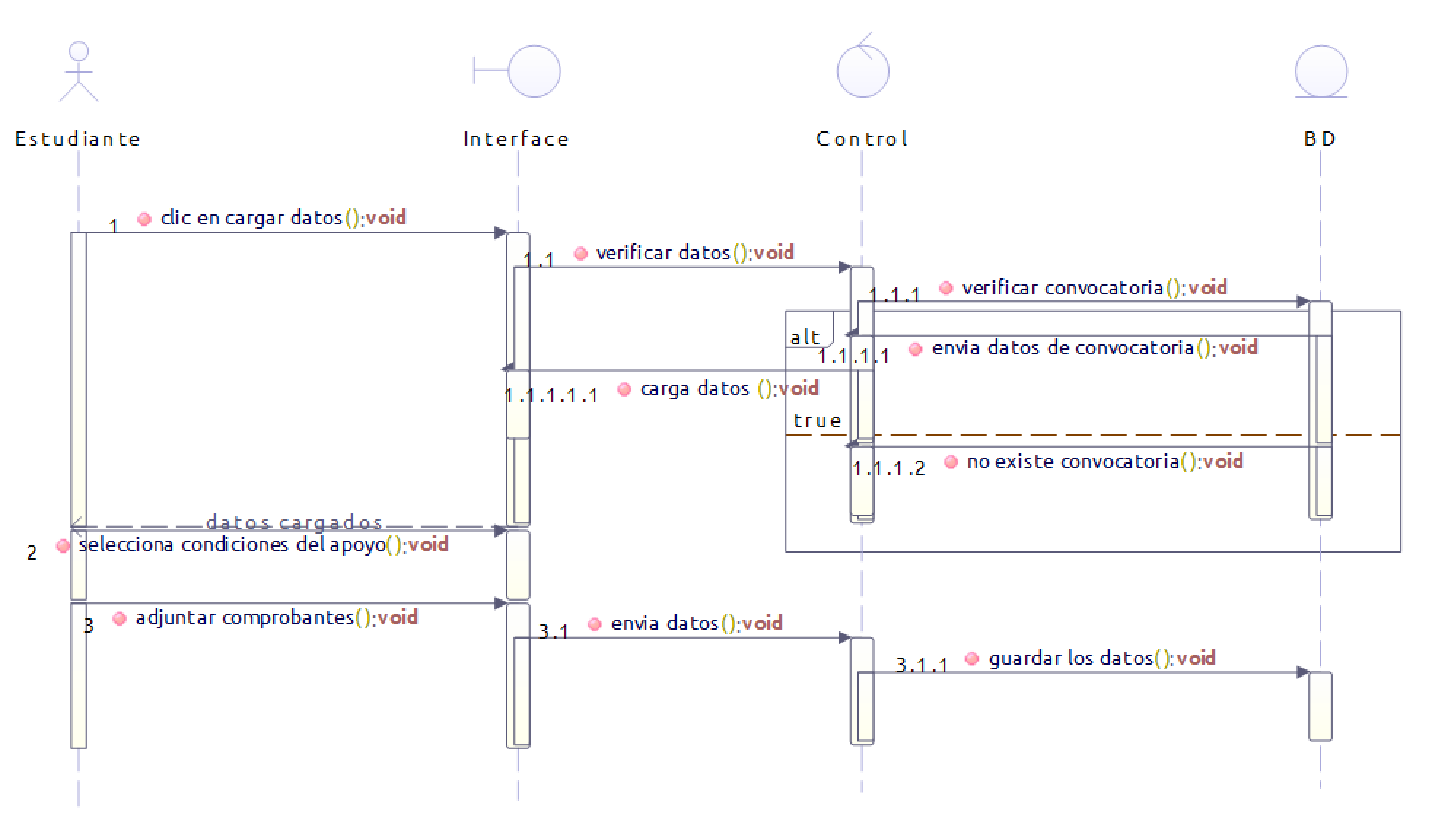
\includegraphics[width=1.3\linewidth]{uml/SecSolConv}
	\caption{Solicitud para registrarse a una convocatoria}
	\label{fig:Solicitud para convocatoria}
	\end{figure}

	\begin{figure}[th!]
	\centering
	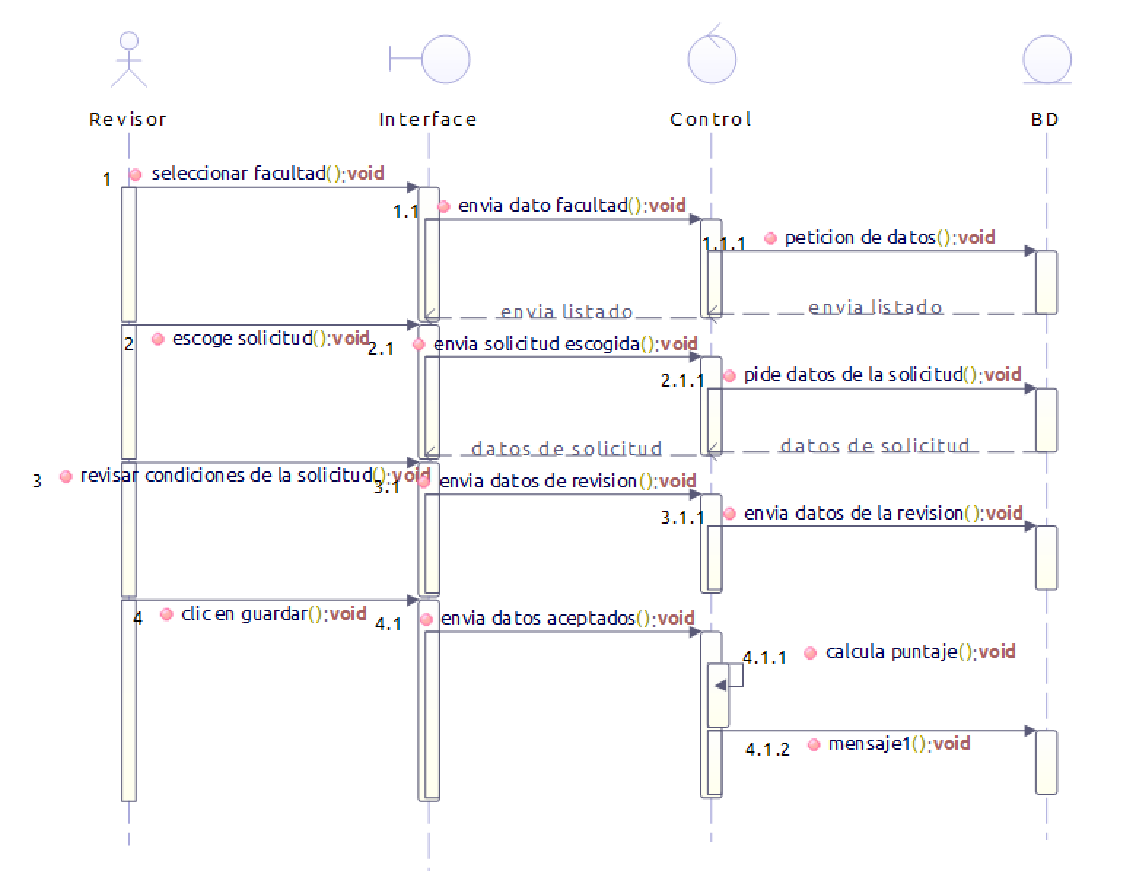
\includegraphics[width=1.4\linewidth]{uml/SecVerifSolConv}
	\caption{Verificar solicitud a una convocatoria}
	\label{fig:Verificar solicitud a una convocatoria}
	\end{figure}
\clearpage

\newpage




\subsection{Diagrama de Comunicación}


\begin{figure}[th!]
	\centering
	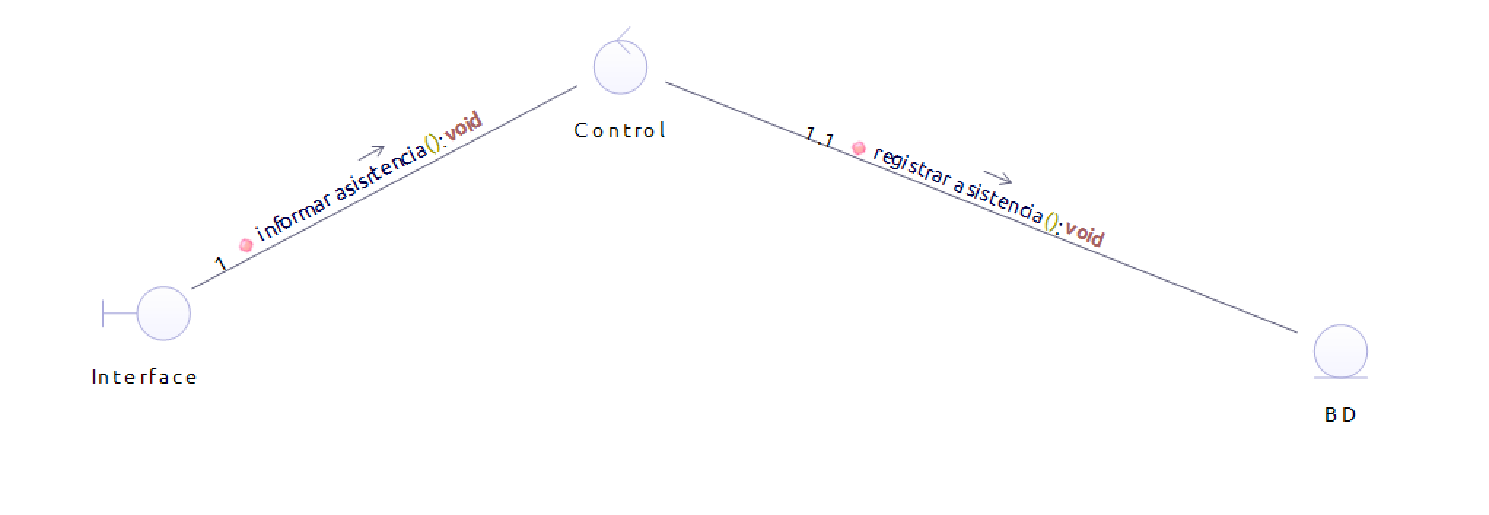
\includegraphics[width=0.9\linewidth]{uml/Comunicacion/ComAsist}
	\caption{Diagrama de Asistencia}
	\label{fig:Diagrama de Asistencia}
\end{figure}

\begin{figure}[th!]
	\centering
	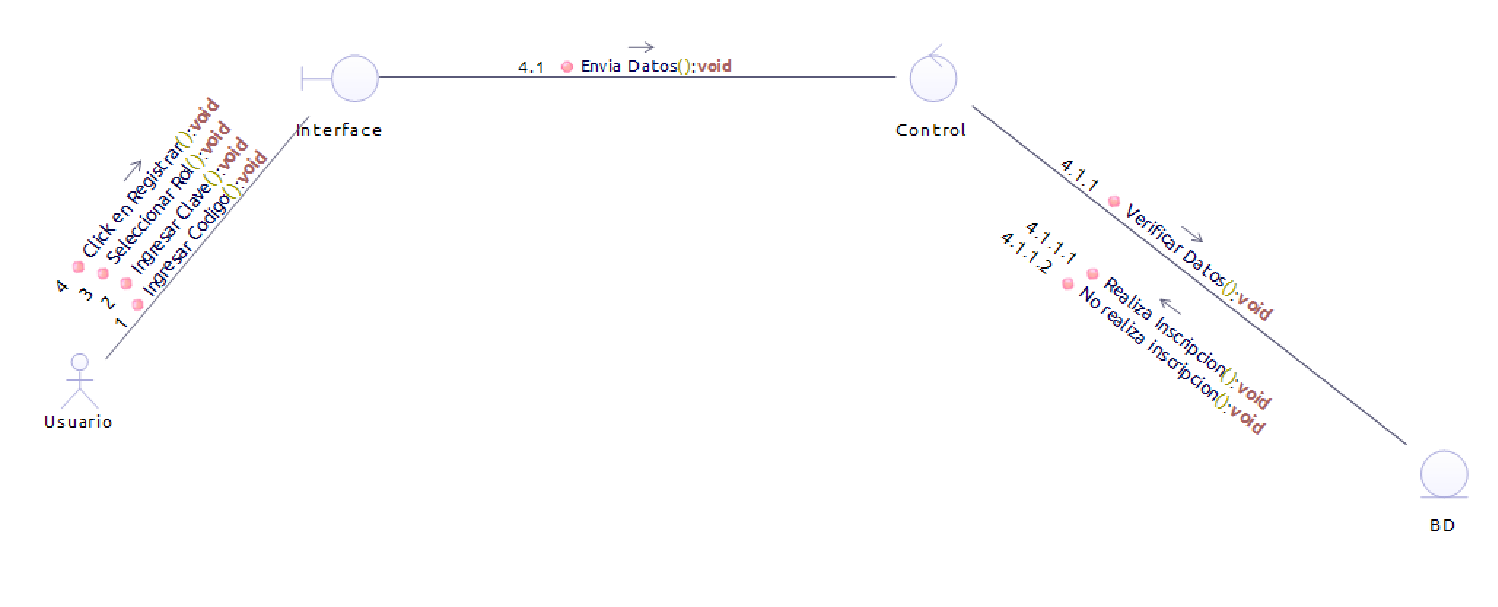
\includegraphics[width=1.1\linewidth]{uml/Comunicacion/ComReguU}
	\caption{Registro del Usuario}
	\label{fig:Registro del Usuario}
\end{figure}

\begin{figure}[th!]
	\centering
	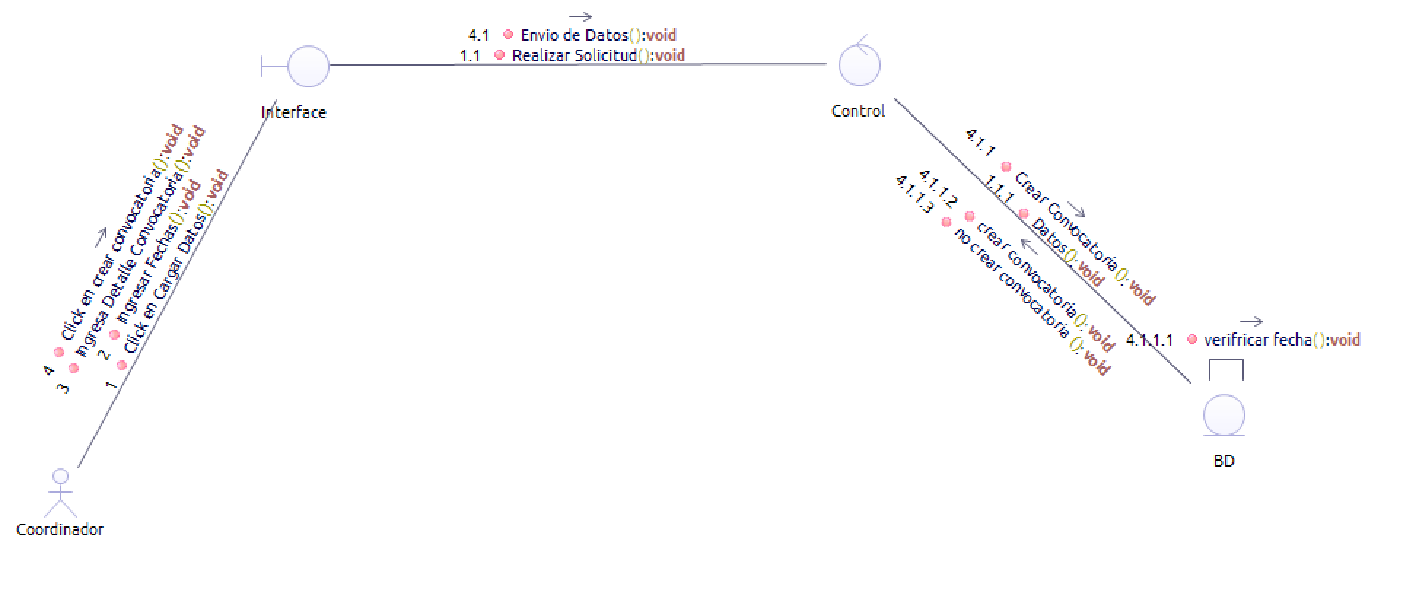
\includegraphics[width=1.4\linewidth]{uml/Comunicacion/ComCreConv}
	\caption{Crear convocatoria del apoyo}
	\label{fig:Crear convocatio del apoyo}
\end{figure}
\clearpage
\begin{figure}[th!]
	\centering
	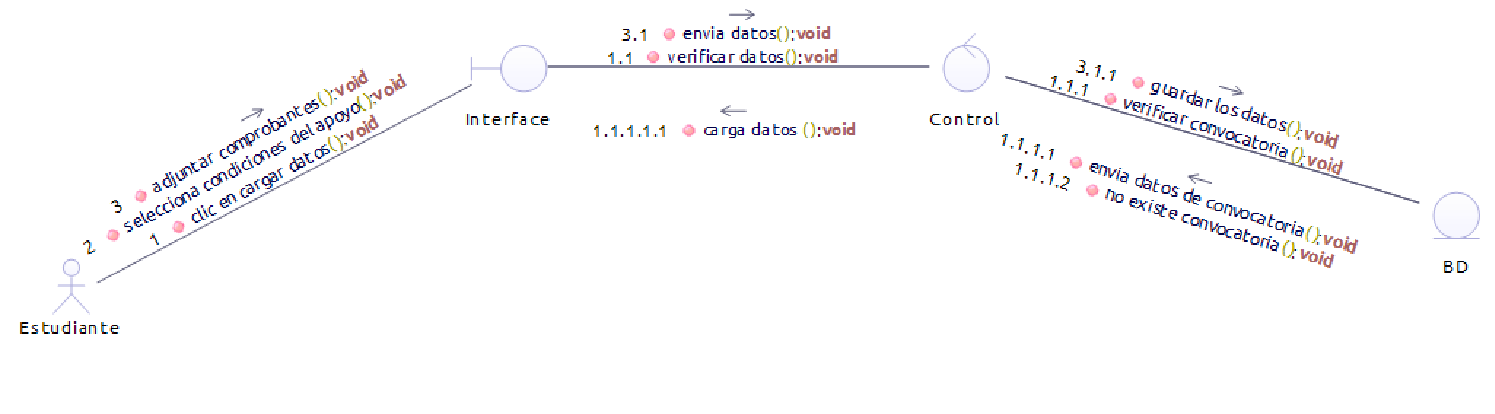
\includegraphics[width=1.2\linewidth]{uml/Comunicacion/ComSoliConv}
	\caption{Solicitud para registrarse a una convocatoria}
	\label{fig:Solicitud para convocatoria}
\end{figure}

\begin{figure}[th!]
	\centering
	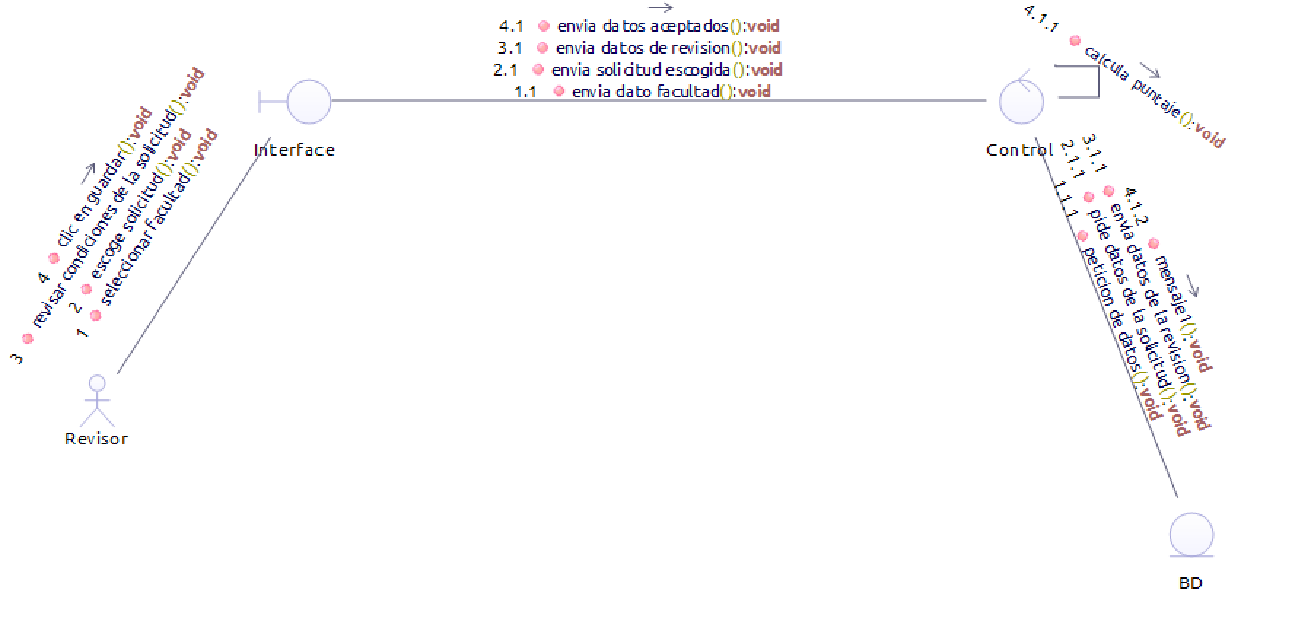
\includegraphics[width=1.2\linewidth]{uml/Comunicacion/ComVer}
	\caption{Verificar solicitud a una convocatoria}
	\label{fig:Verificar solicitud a una convocatoria}
\end{figure}

\clearpage

%%%\subsection{Diagrama de Temporización}

%%\newpage

%%\section{Diagramas de Actividades}

%%\newpage

%%\section{Diagramas de Actividades}

%%\newpage

%%%\section{Diagramas de Workflow}

%%\newpage

%%\section{Diagramas de Descripción de la Interacción}

%%\newpage
